% Copyright (c) 2017 Ongun Kanat <ongun.kanat@gmail.com>
% Permission is hereby granted, free of charge, to any person obtaining a copy of 
% this software and associated documentation files (the "Software"), to deal in 
% the Software without restriction, including without limitation the rights to 
% use, copy, modify, merge, publish, distribute, sublicense, and/or sell copies of 
% the Software, and to permit persons to whom the Software is furnished to do so, 
% subject to the following conditions:
% 
% The above copyright notice and this permission notice shall be included in all 
% copies or substantial portions of the Software.
% 
% THE SOFTWARE IS PROVIDED "AS IS", WITHOUT WARRANTY OF ANY KIND, EXPRESS OR 
% IMPLIED, INCLUDING BUT NOT LIMITED TO THE WARRANTIES OF MERCHANTABILITY, FITNESS 
% FOR A PARTICULAR PURPOSE AND NONINFRINGEMENT. IN NO EVENT SHALL THE AUTHORS OR 
% COPYRIGHT HOLDERS BE LIABLE FOR ANY CLAIM, DAMAGES OR OTHER LIABILITY, WHETHER 
% IN AN ACTION OF CONTRACT, TORT OR OTHERWISE, ARISING FROM, OUT OF OR IN 
% CONNECTION WITH THE SOFTWARE OR THE USE OR OTHER DEALINGS IN THE SOFTWARE.

% 12pt and ISO A4 paper with title page add notitlepage for otherwise
\documentclass[a4paper, 12pt, titlepage]{article}

% Margins and page size
\usepackage[a4paper,top=2.5cm,bottom=2.5cm,left=3.3cm,right=2.2cm]{geometry}

% Page headers are set to top right
\usepackage{fancyhdr}
\pagestyle{fancy}
\renewcommand{\footrulewidth}{0pt} % clear rulers
\renewcommand{\headrulewidth}{0pt}
\lhead{} % Empty left header
\rhead{\thepage} % Page number at the right header
\cfoot{} % Clear center of the footer

% Use American English for dates etc.
%\usepackage[american]{babel}
% If document is in Turkish then use
% \usepackage[turkish]{babel}
% or for both
% \usepackage[turkish,american]{babel}

% Indent at section beginnings
%\usepackage{indentfirst}

% utf-8 support
\usepackage[utf8]{inputenc}

% Graphics for PDFTeX
\usepackage[pdftex]{graphicx}

% Figure placement
\usepackage{float}

% An enumeration package for flexible enumeration
\usepackage{enumitem}

% For fitting tables into the page width
\usepackage{makecell}
\renewcommand{\theadalign}{cc} % Centering and at the middle
\renewcommand{\theadfont}{\bfseries} % Bold table headers

% Helvetica Sans-serif fonts
\usepackage{helvet}
\usepackage{sectsty}
\allsectionsfont{\normalfont\sffamily\bfseries}
\sectionfont{\fontsize{18pt}{21.6pt}\sffamily\bfseries}
\subsectionfont{\fontsize{16pt}{19.2pt}\sffamily\bfseries}
\subsubsectionfont{\fontsize{14pt}{16.8pt}\sffamily\bfseries}

% Courier monospace font
\usepackage{courier}

% Table of contents dot fill, sans serif header and name change
\usepackage{tocloft}
\renewcommand{\cftsecleader}{\cftdotfill{\cftdotsep}}
\tocloftpagestyle{fancy}
\renewcommand{\cfttoctitlefont}{\sffamily\Large\bfseries}
\setlength{\cftbeforesecskip}{6pt}
\renewcommand{\contentsname}{Table of Contents}

% Links, both local and external
\usepackage{hyperref}
\hypersetup{
	unicode=true,
	colorlinks=true,
	urlcolor=blue,
	citecolor=black,
	menucolor=black,
	linkcolor=black
}

% Figure captions are bold
\usepackage[labelfont=bf,font=sf]{caption}

% Pseudocode from algorithmicx package
\usepackage{algorithmicx}
\usepackage{algpseudocode}
\usepackage[section,boxed]{algorithm}
\captionsetup[algorithm]{labelfont=bf,font=sf,justification=centering,position=top}

% Listings for implemented code
\usepackage{listings}
\lstset{basicstyle=\ttfamily,frame=lines,tabsize=4}
\renewcommand{\lstlistingname}{Listing}

% A powerful math notation package
\usepackage{amsmath}

% Title, author and date info
\title{Graduation Project}
\author{Besim Ongun Kanat}
\date{June 2017}

\begin{document}
\numberwithin{figure}{section}
\numberwithin{table}{section}
\numberwithin{lstlisting}{section}

\begin{titlepage}
    \bfseries % Make all text bold in this environment
    \sffamily % Similarly select sans-serif font
	\begin{center}
		\LARGE{\textbf{ISTANBUL TECHNICAL UNIVERSITY \\ 
               FACULTY OF COMPUTER AND INFORMATICS} } \\
		\vspace{5.5cm}
		\LARGE{PROJECT TITLE}  \\
		\vspace{4.5cm}
		\Large{Graduation Project} \\
        \vspace{0.5cm}
		\Large{Besim Ongun Kanat} \\
     	\Large{150120047} \\
        \vspace{4cm}
        \large{Department: Computer Engineering} \\
        \large{Division: Computer Engineering} \\
        \vspace{1.5cm}
        \large{Advisor: Assoc. Prof. Dr. Sanem Sarıel} \\
		\vspace{\fill} % Fill out until the page end
		\large{\normalfont \sffamily June 2017}
	\end{center}
\end{titlepage}

\pagenumbering{Roman} % Capital roman numerals as page numbers
\newpage
\section*{Özgünlük Bildirisi}
\begin{enumerate}
    \item Bu çalışmada, başka kaynaklardan yapılan tüm alıntıların, ilgili kaynaklar \\ referans gösterilerek açıkça belirtildiğini,
    \item Alıntılar dışındaki bölümlerin, özellikle projenin ana konusunu oluşturan teorik çalışmaların ve yazılım/donanımın benim tarafımdan yapıldığını
    bildiririm.
\end{enumerate}
\vspace{1em}
İstanbul, TARİH
\vspace{3em}\\Besim Ongun Kanat

\newpage
\section*{Acknowledgments}

\newpage
\section*{English Project Title}
\centerline{\large\bfseries (Summary)}


\newpage
\section*{Türkçe Proje Başlığı}
\centerline{\large\bfseries (Özet)}

\newpage
\tableofcontents
\newpage

% For the ones who doesn't know: 1,2,..9 called West Arabic numbers
\pagenumbering{arabic}
\section{Introduction}
In November 1936 Alan Turing published his groundbreaking paper which creates foundations of computer science \cite{turing1937computability}. It was the Big-Bang of the computer science that created a new universe from dusty works of his ancestors.
\newpage
\section{Project Description and Plan}
This is the best graduation project ever. In Figure \ref{fig:ganttdiagram} you can see the Gantt diagram of the project.

\begin{figure}[H]
    \centering
    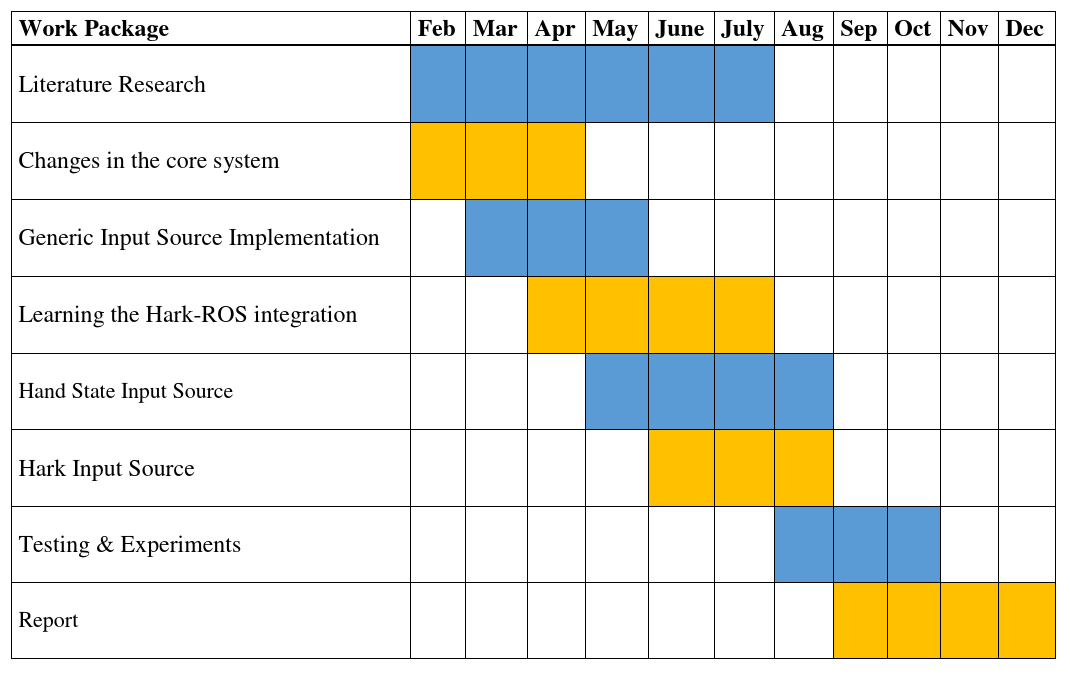
\includegraphics[width=\linewidth]{gantt_diagram}
    \caption{The Gantt diagram of the project}
    \label{fig:ganttdiagram}
\end{figure}

\newpage
\section{Background}
A long long section with many papers.

\newpage
\section{Analysis and Modeling}
After long hours of studying we decided. A* is the best algorithm for searching on the graphs.

\newpage
\section{Design and Implementation}
We implemented the depth first search algorithm as shown in Algorithm \ref{algo:dfs}.
\begin{algorithm}[H]
    \caption{The depth first search algorithm}
    \label{algo:dfs}
    \begin{algorithmic}[1]
        \State \textbf{Graph} $G$
        \State \textbf{Node} $start$
        \Function{Depth-First-Search}{$G$, $start$}
        \State \textbf{Tree} $ T $ \Comment The resulting search tree
        \State \textbf{Stack} $ S $ \Comment An empty stack
        \State \textbf{Set} $ V $ \Comment An empty set of visited nodes
        \State \Call{set-root}{$ T $,$ current $}
        \State \Call{push}{$ S $,$ start $}
        \While{\Call{not-empty}{S}}
        \State $current \gets$ \Call{pop}{$ S $}
        \If{\textbf{not} \Call{Contains}{$ V $, $ current $} }
        \State \Call{insert}{$ V $, $ current $}
        \ForAll{$ n $ : \Call{neighbors}{$ current $} }
        \State \Call{push}{$ S $, $ n $}
        \State \Call{insert-sub-node}{$ T $, $ current $, $ n $}
        \Comment Insert node to subtree of $ current $
        \EndFor
        \EndIf
        \EndWhile
        \State \Return $ T $
        \EndFunction
    \end{algorithmic}
\end{algorithm}

\newpage
\section{Testing and Evaluation}
We compared the performance of the graph search algorithms. The results can be seen in the Table \ref{tbl:results}.

\begin{table}[H]
    \caption{Performance test results of the graph search algorithms}
    \label{tbl:results}
    \centering
    \begin{tabular}{|c|r|r|r|} 
        \hline 
        \thead{Algorithm} & \thead{Number of \\ Generated Nodes} & \thead{Number of \\ Nodes Expanded} & \thead{Max Number of \\ Nodes in The Frontier} \\ 
        \hline 
        BFS &  77480 & 6340 & 71142 \\ 
        \hline 
        DFS & 820 & 88 & 760 \\ 
        \hline 
        A* & 376 & 33 & 338 \\ 
        \hline 
    \end{tabular}
\end{table}

\newpage
\section{Conclusion and Future Work}
We tested algorithms and decided that future is bright.

\newpage
\bibliographystyle{IEEEtran}
\bibliography{references.bib} 

\end{document}
